%        File: doc.tex
%     Created: Mon Aug 08 10:00 AM 2022 E
% Last Change: Mon Aug 08 10:00 AM 2022 E
%
\documentclass[a4paper]{report}
\maxdeadcycles=200
\usepackage[section]{placeins}
\usepackage{mathtools}
\usepackage{amsmath}
\usepackage{pgffor}
\usepackage{booktabs}
\begin{document}
\begin{titlepage}
    \begin{center}
        \vspace*{1cm}

        \textbf{Analytical Solution for Duct Mode Propagation in %
        Uniform Flow} 

        \vspace{0.5cm}
        Swirl Validation

        \vspace{1.5cm}

        \textbf{Jeff Severino}

        \vfill


        This document shows the analytical duct mode solution as well as a
        numerical comparison.
        \vspace{0.8cm}

        % \includegraphics[width=0.4\textwidth]{university}

        Mechanical, Industrial, Manufacturing Engineering Department\\
        University Of Toledo\\
        Toledo, OH\\
        \today

    \end{center}
\end{titlepage}
\section{Introduction - Turbomachinery Noise}
Turbomachinery noise generation occurs from pressure fluctuations from the series 
of fans within it's annular duct. While the jet that is produced from this stream
of air freely radiates to the observer, the pressure fluctuations 
produced from the rotor may or may not propagate out of the inlet and exhaust and 
radiate to the observer. The production of this propagation can be characterized
by standing waves referred to as modes, in particular, duct modes because 
the mode itself is dependent on the geometry of the column of air within the 
annular duct, as well as the speed of the flow moving through it
\newpage

\section{Duct Mode Theory}
The pressure field within a duct is governed by the convective wave equation, a
second order ODE as a function of radius. 

% Goldstein's \textit{Aeroacoustics} 
% shows that the wave equation can be obtained by taking the divergence of the
% momentum equation and subtracting the material derivative of the continuity 
% equation, however, the same equation can be obtained by resubstitution of the 
% continuity and momentum equations into the energy equations after the fluctuations 
% have also been substituted for the primative variables. (See Appendix for derivation)

The solution of the convective wave equation are eigenvalues and eigenvectors 
which may or may not correspond to acoustic disturbances fall into two groups.  
One group corresponding to the acoustics propagation and the other group 
corresponding to the convection speed of the flow. Both are modes that are a
result from the pressure distribution from within the cylindrical domain.  

\subsection{ Analytic Solution: Axial wavenumbers and Pressure Modes}

Modes can be categorized based on the sign of the axial wavenumber and if it is
complex in value. For example, for the uniform axial flow case, propagating modes
are defined by axial wavenumbers, $k_x$, that have a real-part only, yielding 
the assumed fluctuation to resemble Euler's Formula ($e^{ik_x x}$). On the other 
hand, if the $k_x$ is complex, then the mode will resemble an exponentially decaying
function since the imaginary number cancels, leaving a minus sign in front of
the axial wavenumber. These two distinctions are referred to as ``cut-on'' and 
``cut-off'' in the field of ducted sound propagation. Furthermore, the sign of 
the imaginary part will change the direction of the mode's decay. If $k_x$ is 
positive, the decay rate occurs in the negative direction. Conversely, if $k_x$ 
is negative, the decay occurs in the positive direction. The axial wavenumber
for uniform axial flow in a hollow duct is,

\begin{equation}
    k_x  = \frac{- M_x k \pm \sqrt{k^2 - ( 1 - M_x^2) J_{m,n}'^2 }}{\left( 1 - M_x^2 \right)}.
    \label{eqn:ax_wavenumb}
\end{equation}

where $M_x$ is the axial Mach number, $k$ is the temporal (referred to as reduced)
frequency, and $J_{m,n}'$ is the derivative of the Bessel function of the first kind.  
The $\pm$ accounts for both upstream and downstream modes.

The condition for propagation is such that the axial wavenumber is larger than 
a ``cut-off'' value

\begin{equation}
    k_{x,real}  = \frac{\pm M_x k }{\left( M_x^2 - 1 \right)}.
    \label{eqn:cuton}
\end{equation}

Every term that is being raised to the one half i.e. square rooted must 
be larger than zero to keep axial wavenumber from being imaginary. The mode 
will propagate or decay based on this condition. 

\subsection{Methods}
Bessel's Function,

\begin{equation}
    R(r) = A J_0 (k_r r) + B Y_0(k_r r ) 
    \label{eqn:besselsfun}
\end{equation}
where $J_0$ and $Y_0$ are Bessel's functions of the first 
and second kind, and $A$ and $B$ are arbitrary constants. 
Both functions reduce as $k_r r$ gets large. The Bessel function of the second
kind is unbounded as $k_r r$ goes to zero. 

For a hard-walled duct, the radial velocity component is zero at the 
boundaries $r_{min}$ and $r_{max}$. 

\begin{equation}
    \frac{dR(r)}{dr}\Bigr|_{r = r_{max}}  =%
    \frac{dR(r)}{dr}\Bigr|_{r = r_{min}}   = 0
    \label{eqn:besselBC}
\end{equation}
In the case of a hollow duct, there is no
minimum radius, therefore the wall boundary condition only applies at $r_{max}$.


Since the solution must be finite as $k_r r$ approaches zero, it can be observed
that $Y_0$ approaches infinity. Since this would yield in a trivial solution, the 
coefficient $B = 0$, which reduces \ref{eqn:besselsfun} to,

\begin{equation}
    R(r) = A J_0 (k_r r) 
    \label{eqn:besselsfunCylinder}
\end{equation}

Taking the derivative 
with respect to $r$ yields,

\begin{equation}
    \frac{dR(r)}{dr}\Bigr|_{r} = A J'_0 (k_r r)  = 0
    \label{eqn:besselsfunderivaTive}
\end{equation}
The boundary condition requires the Bessel function be zero at a hard wall.
The terms inside of the Bessel function would then correspond to values along 
the domain, $k_r r$,  which satisfy our equation.  Let $k_r r = \alpha_{m,n}$ 
where, $alpha$ represents the zeros of the Bessel function, and 
$m$ corresponds to the azimuthal mode order and $n$ represents the radial mode
order, i.e. the index for the number of zero crossings in the 
derivative of the Bessel function of the first kind. 

Therefore,


\begin{align}
    \frac{dR}{dr}\Bigr|_{r = r_{max}} = A J'_0 (k_r r_{max})  = 0 \\
    (k_r r_{max})  = 0 
\end{align}
Recalling $\alpha_{m,n}$


\begin{align}
    (k_r r_{max})  = \alpha_{m,n} \\
    k_r = \alpha_{m,n}/r_{max}
\end{align}

For annular ducts, $r_{min}$ is no longer zero, therefore $B$ cannot be removed
since $Y_0'$ has finite values as $k_r r $ increases.

\begin{equation}
    \frac{dR}{dr}\Bigr|_{r} = A J'_0 (k_r r) + B Y'_0(k_r r ) 
    \label{eqn:besselsfunderivaTive}
\end{equation}
Applying boundary conditions to both inner and outer walls at $r_{min}$ and $r_{max}$

\begin{equation}
    \frac{dR}{dr}\Bigr|_{r=r_{min}} = A J'_0 (k_r r_{min}) + B Y'_0(k_r r_{min}) 
\end{equation}

\begin{equation}
    \frac{dR}{dr}\Bigr|_{r=r_{max}} = A J'_0 (k_r r_{max}) + B Y'_0(k_r r_{max}) 
\end{equation}

defining $\beta = \frac{B}{A}$,

\begin{equation}
    \frac{dR}{dr}\Bigr|_{r=r_{min}} =  J'_0 (k_r r_{min}) + \beta Y'_0(k_r r_{min}) 
\end{equation}

\begin{equation}
    \frac{dR}{dr}\Bigr|_{r=r_{max}} =  J'_0 (k_r r_{max}) + \beta Y'_0(k_r r_{max}) 
\end{equation}

Defining,

\begin{align*}
    k_r^{n+1} = k_r^n + \Delta k_r \\
    \beta^{n+1} = \beta^n + \Delta \beta 
\end{align*}
And substituting into the boundary condition expressions,
\begin{equation}
    \frac{dR}{dr}\Bigr|_{r=r_{min}} =  J'_0 (k_r^{n+1} r_{min}) + \beta^{n+1} Y'_0(k_r^{n+1} r_{min}) 
\end{equation}

\begin{equation}
    \frac{dR}{dr}\Bigr|_{r=r_{max}} =  J'_0 (k_r^{n+1} r_{max}) + \beta^{n+1} Y'_0(k_r^{n+1} r_{max}) 
\end{equation}



% \begin{equation}
%     p' = f(r) e^{i(m \theta + k x - \omega t)}
% \end{equation}
% Recall thaT the mode is of the 
% form 
% \begin{equation}
%     e^{i k_x x}
%     \label{eqn:fluctuationexample}
% \end{equation}
% if $k_x$ has a real part, $k_{x,real}$ and an imaginary part $i k_{x,imag}$ 
% then,

% \begin{align}
%     &= e^{i k_x x} \\
%     &= e^{i (k_{x,real}+ i k_{x,imag}) x} \\
%     &= \underbrace{e^{i k_{x,real}x}}_{\textit{amplitude}} \underbrace{e^{- k_{x,imag} x}}_{\textit{exponential decay}} 
% \end{align}

% Although the ``cut-off'' decay to nearly zero rapidly, the rate at which this occured
% was not much of a concern earlier on in turbomachinery design. As nacelles 
% continue to grow shorter, a mode that is ``cut-off'' may make it outside the duct.

% For this work a desired amplitude was arbitrarily chosen for a mode, $y_{desired}$
% and then the axial location at which this occurred, $x_{desired}$ which 
% can be compared against a desired length for a nacelle.  
% Since SWIRL assumes an infinitely long duct, there is nothing limiting the 
% modes propagation with respect to nacelle length. For example, if the 
% desired amplitude is one percent, then $x_{desired}$ is $0.46$, 

% \begin{align*}
%     0.01 &=  e^{-10 x_{desired}},\\
%     -\frac{ln|0.01|}{10} &=  x_{desired},\\
%     -\frac{ln|0.01|}{10} &= 0.4605170185988091 .
% \end{align*}


 % \begin{figure}
 %     \centering
 %     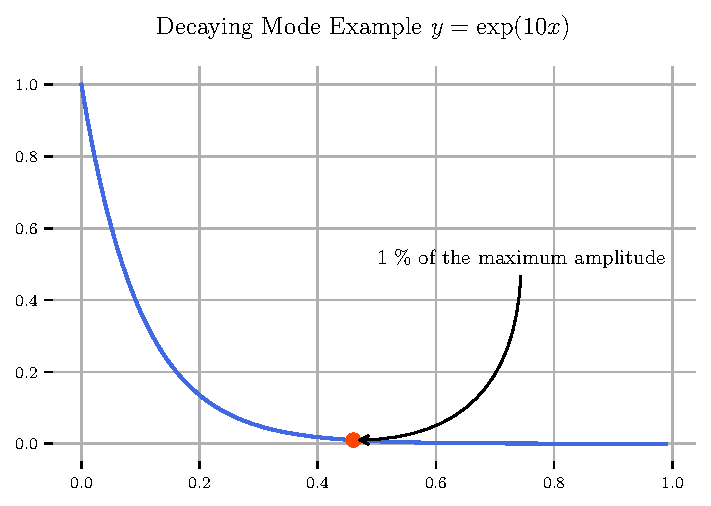
\includegraphics[width=\textwidth]{/home/jeff-severino/SWIRL/CodeRun/04-plotReport/tex-outputs/desired_cut_off_location_1_percent_of_max.pdf}
 %     \caption{Decaying mode with $k_x = 0 + 10j$ and unit amplitude. One percent
 %     of the maximum amplitude is identified for nacelle length comparison}
 %     \label{fig:decaying_mode_with_1_percent_amp}
 % \end{figure}
 
 
% In general,
% \begin{align*}
 %    y_{desired} &=  e^{-k_{x,imag} x_{desired} }\\
 %    -\frac{ln|y_{desired}|}{k_{x,imag}} &=  x_{desired}
% \end{align*}
\section{Analytical Test Case}
The results present a comparison of analytical and numerical solutions for a
uniform flow, hard-wall, cylindrical duct for six grids. The physical 
parameters for this test case are reporte in Table 1. The grid points were
doubled each iteration and a starting grid of 33 points was chosen. The 
first five radial modes were chosen in order to get a group of modes that were cut
on and cut off. The case number's are used as identifiers for each 
mode propagating up or downstream. In the event that a spurious mode is identified,
the case number will index it.  The number of cut off modes was also constrained
by setting a maximum value for the imaginary part of the axial wavenumber. 
While this magnitude is currently arbitrary, the value could be correlated to a
desired decay rate for the corresponding mode. Each of the axial wavenumber's 
radial mode for each grid in also reported. The same test case was ran twice using 
second and fourth order central schemes for the radial derivatives.  The 
approximate rate of convergence is also reported for both numerical schemes.
\begin{table}[!h]
    \centering
    \begin{tabular}{|l|l|}
        \hline
        $\sigma$ & \textit{0.0} \\ \hline
        $k$      & \textit{10}   \\ \hline
        $m$      & \textit{2}    \\ \hline
        $M_x$    & \textit{0.3}  \\ \hline
    \end{tabular}
    \caption{Validation test case parameters, Uniform Flow Hard-wall Cylindrical%
    Duct} 
\end{table}

\newpage
\subsection{Axial Wavenumber}
\foreach \i in {33,66,132,264,528,1056}
{
    \begin{figure}
        \centering
        \includegraphics[width=\textwidth]
        {../figures/second_order_wavenumber_grid_\i.pdf}
    \caption{ Second Order, Analytical Solution vs Numerical Approximation using \i\  points}
    \end{figure}
}
\foreach \i in {33,66,132,264,528,1056}
{
    \begin{figure}
        \centering
        \includegraphics[width=\textwidth]
        {../figures/fourth_order_wavenumber_grid_\i.pdf}
    \caption{ Fourth Order, Analytical Solution vs Numerical Approximation using \i\  points}
    \end{figure}
}

\clearpage
\subsection{Propagating Radial Modes}

\subsubsection{Second Order, Radial Mode 0}
\foreach \i in {0,...,1}
{
    \foreach \j in {33,66,132,264,528,1056} 
    {
        \begin{figure}
            \centering
            \includegraphics[width=\textwidth]
            {../figures/second_order_radial_mode_0_test_case_number_\i_grid_\j.pdf}
            \caption{Second Order, Case number \i, \j points}
            \label{fig:analytical_bessel_function}
        \end{figure}
        \begin{figure}
            \centering
            \includegraphics[width=\textwidth]
            {../figures/second_order_radial_mode_error_0_test_case_number_\i_grid_\j.pdf}
            \caption{Second Order, Case number \i, \j points}
            \label{fig:analytical_bessel_function}
        \end{figure}
    }
}
\clearpage

% \stop

\subsubsection{ Fourth Order, Radial Mode 0}
\foreach \i in {0,...,1}
{
    \foreach \j in {33,66,132,264,528,1056} 
    {
        \begin{figure}
            \centering
            \includegraphics[width=\textwidth]
            {../figures/fourth_order_radial_mode_0_test_case_number_\i_grid_\j.pdf}
            \caption{Fourth Order, Case number \i, \j points}
            \label{fig:analytical_bessel_function}
        \end{figure}
        \begin{figure}
            \centering
            \includegraphics[width=\textwidth]
            {../figures/fourth_order_radial_mode_error_0_test_case_number_\i_grid_\j.pdf}
            \caption{Fourth Order, Case number \i, \j points}
            \label{fig:analytical_bessel_function}
        \end{figure}
    }
}
\clearpage
\subsubsection{Second Order, Radial Mode 1}
\foreach \i in {0,...,1}
{
    \foreach \j in {33,66,132,264,528,1056} 
    {
        \begin{figure}
            \centering
            \includegraphics[width=\textwidth]
            {../figures/second_order_radial_mode_1_test_case_number_\i_grid_\j.pdf}
            \caption{Second Order, Case number \i, \j points}
            \label{fig:analytical_bessel_function}
        \end{figure}
        \begin{figure}
            \centering
            \includegraphics[width=\textwidth]
            {../figures/second_order_radial_mode_error_1_test_case_number_\i_grid_\j.pdf}
            \caption{Second Order, Case number \i, \j points}
            \label{fig:analytical_bessel_function}
        \end{figure}
    }
}

\clearpage
\subsubsection{Fourth Order, Radial Mode 1}
\foreach \i in {0,...,1}
{
    \foreach \j in {33,66,132,264,528,1056} 
    {
        \begin{figure}
            \centering
            \includegraphics[width=\textwidth]
            {../figures/fourth_order_radial_mode_1_test_case_number_\i_grid_\j.pdf}
            \caption{Fourth Order, Case number \i, \j points}
            \label{fig:analytical_bessel_function}
        \end{figure}
        \begin{figure}
            \centering
            \includegraphics[width=\textwidth]
            {../figures/fourth_order_radial_mode_error_1_test_case_number_\i_grid_\j.pdf}
            \caption{Fourth Order, Case number \i, \j points}
            \label{fig:analytical_bessel_function}
        \end{figure}
    }
}

\clearpage
\subsubsection{Second Order, Radial Mode 2}
\foreach \i in {0,...,1}
{
    \foreach \j in {33,66,132,264,528,1056} 
    {
        \begin{figure}
            \centering
            \includegraphics[width=\textwidth]
            {../figures/second_order_radial_mode_2_test_case_number_\i_grid_\j.pdf}
            \caption{Second Order, Case number \i, \j points}
            \label{fig:analytical_bessel_function}
        \end{figure}
        \begin{figure}
            \centering
            \includegraphics[width=\textwidth]
            {../figures/second_order_radial_mode_error_2_test_case_number_\i_grid_\j.pdf}
            \caption{Second Order, Case number \i, \j points}
            \label{fig:analytical_bessel_function}
        \end{figure}
    }
}

\clearpage
\subsubsection{Fourth Order, Radial Mode 2}
\foreach \i in {0,...,1}
{
    \foreach \j in {33,66,132,264,528,1056} 
    {
        \begin{figure}
            \centering
            \includegraphics[width=\textwidth]
            {../figures/fourth_order_radial_mode_2_test_case_number_\i_grid_\j.pdf}
            \caption{Fourth Order, Case number \i, \j points}
            \label{fig:analytical_bessel_function}
        \end{figure}
        \begin{figure}
            \centering
            \includegraphics[width=\textwidth]
            {../figures/fourth_order_radial_mode_error_2_test_case_number_\i_grid_\j.pdf}
            \caption{Fourth Order, Case number \i, \j points}
            \label{fig:analytical_bessel_function}
        \end{figure}
    }
}


\clearpage
\subsubsection{Second Order, Radial Mode 3}
\foreach \i in {0,...,1}
{
    \foreach \j in {33,66,132,264,528,1056} 
    {
        \begin{figure}
            \centering
            \includegraphics[width=\textwidth]
            {../figures/second_order_radial_mode_3_test_case_number_\i_grid_\j.pdf}
            \caption{Second Order, Case number \i, \j points}
            \label{fig:analytical_bessel_function}
        \end{figure}
        \begin{figure}
            \centering
            \includegraphics[width=\textwidth]
            {../figures/second_order_radial_mode_error_3_test_case_number_\i_grid_\j.pdf}
            \caption{Second Order, Case number \i, \j points}
            \label{fig:analytical_bessel_function}
        \end{figure}
    }
}

\clearpage
\subsubsection{Fourth Order, Radial Mode 3}
\foreach \i in {0,...,1}
{
    \foreach \j in {33,66,132,264,528,1056} 
    {
        \begin{figure}
            \centering
            \includegraphics[width=\textwidth]
            {../figures/fourth_order_radial_mode_3_test_case_number_\i_grid_\j.pdf}
            \caption{Fourth Order, Case number \i, \j points}
            \label{fig:analytical_bessel_function}
        \end{figure}
        \begin{figure}
            \centering
            \includegraphics[width=\textwidth]
            {../figures/fourth_order_radial_mode_error_3_test_case_number_\i_grid_\j.pdf}
            \caption{Fourth Order, Case number \i, \j points}
            \label{fig:analytical_bessel_function}
        \end{figure}
    }
}



\clearpage
\subsubsection{Second Order, Radial Mode 4}
\foreach \i in {0,...,1}
{
    \foreach \j in {33,66,132,264,528,1056} 
    {
        \begin{figure}
            \centering
            \includegraphics[width=\textwidth]
            {../figures/second_order_radial_mode_4_test_case_number_\i_grid_\j.pdf}
            \caption{Second Order, Case number \i, \j points}
            \label{fig:analytical_bessel_function}
        \end{figure}
        \begin{figure}
            \centering
            \includegraphics[width=\textwidth]
            {../figures/second_order_radial_mode_error_4_test_case_number_\i_grid_\j.pdf}
            \caption{Second Order, Case number \i, \j points}
            \label{fig:analytical_bessel_function}
        \end{figure}
    }
}

\clearpage
\subsubsection{Fourth Order, Radial Mode 4}
\foreach \i in {0,...,1}
{
    \foreach \j in {33,66,132,264,528,1056} 
    {
        \begin{figure}
            \centering
            \includegraphics[width=\textwidth]
            {../figures/fourth_order_radial_mode_4_test_case_number_\i_grid_\j.pdf}
            \caption{Fourth Order, Case number \i, \j points}
            \label{fig:analytical_bessel_function}
        \end{figure}
        \begin{figure}
            \centering
            \includegraphics[width=\textwidth]
            {../figures/fourth_order_radial_mode_error_4_test_case_number_\i_grid_\j.pdf}
            \caption{Fourth Order, Case number \i, \j points}
            \label{fig:analytical_bessel_function}
        \end{figure}
    }
}


\section{Discussion}






\end{document}


